The biggest benefit of the extended SFA rate in \eqref{eq:sfa_rate_improved} is not only that it incorporates more physical effects than standard SFA, but also that, with certain `tricks,’ the influence of different physical effects on the ionization dynamics can be observed. This is preferable to simply presenting a modified rate that yields better results without understanding \emph{why} it yields better results. Before discussing whether the improvement of the SFA rate was successful, it is first necessary to define what can be learned from this kind of generalization.

The goal is to investigate how the incorporation of excited states and the influence of the laser field on the atom affects the ionization process. Specifically, the focus is on determining whether the Stark shift or the distortion of the ground state has a greater impact on the ionization dynamics. This question is answered in this Chapter.

However, a more significant issue is the previously known considerable discrepancy between the overall ionization yield obtained from SFA simulations and the numerical solution of the TDSE. An extended version of the SFA model could help determine whether this discrepancy arises from simplifications in the dynamics before or after ionization. Unfortunately, a fully satisfactory answer to this question cannot be provided in this thesis, even though the theoretical framework of Chapter 2 allows for such an investigation. This remains a topic for future work. This aspect requires additional investigation in future work.



% In other words, by including the dynamics before ionization, the remaining difference between the SFA and the TDSE will likely be because of the strong field approximation itself.
% If one would simplify both processes, the only shure information is that both results dont match but one dont know what causes it, the neglection of excited states, SFA itself, or something in between.





%%%%%%%%%%%%%%%%%%%%%%
\section{Comparison of Ionization Dynamics with TDSE using TIPTOE}
% \paragraph{Interpretation of extended SFA formula}
% Since the derivation of formula \eqref{eq:sfa_rate_improved} is also one main result of this thesis, I beginn with interpreting the formula. 
\paragraph{Improved Reconstruction of Ionization Dynamics}
The ionization dynamics predicted by the standard SFA approach \cite{Theory_NPS} are first compared with the results from the numerical solution of the TDSE. As shown in \ref{fig:tiptoe_sfa_comparison}(a), the standard SFA generally provides a good reconstruction of the ionization dynamics, though some features are not captured at all\footnote{Note that \eqref{eq:tiptoeprop} is fulfilled and $\delta N(\tau)$ is proportional to the signal pulse.}. In particular, the off-cycle ionization dynamics exhibits a phase shift that does not match the numerical results.

\medskip
This discrepancy serves as the starting point and motivation of this thesis.
To address this, the extended SFA model described in Chapters 2 and 4 was implemented.
As previously mentioned, the coefficients can be determined in two ways: either by solving the TDSE in the subspace of the Hilbert space using the system of ODEs or numerically in the full Hilbert space using a numerical solver (here, tRecX). In \ref{fig:tiptoe_sfa_comparison}(b), the TIPTOE results from both the subspace and full Hilbert space approaches are shown.
Importantly, only the first coefficient and first dipole matrix element are used here. In other words, in \eqref{eq:sfa_rate_improved}, only the first term is considered, i.e., $n_1=n_2=1$.
The same formula was already used for simulating the standard SFA model.
The only difference is that in the extended SFA model for one state, the coefficient $c_0(t)$ is included, meaning all the differences between the standard SFA and extended SFA in \ref{fig:tiptoe_sfa_comparison}(b) are solely due to them.

\medskip
The results indicate that the extended SFA model using coefficients from the full Hilbert space improves the reconstruction of the off-cycle ionization dynamics. Given that only the ground-state coefficients are used and no excited states are included, this represents a significant improvement. Furthermore, as discussed in more detail in Chapter 4, several approximations were made even with the coefficients from the numerical solver.

\medskip
Interestingly, the TIPTOE measurement with coefficients from the subspace does not differ significantly from the standard SFA model.
This suggests that no physical contribution from the coefficients of the wavefunction confined to the subspace of the bound state is captured by TIPTOE in the ionization dynamics.
The consequences of this observation are elaborated in the next paragraph.

\medskip
Additionally, the extended SFA model still appears to lack some physical contributions.
Since \ref{fig:tiptoe_sfa_comparison}(b) does not account for transitions to excited states, this could explain the remaining discrepancies.
Another possible reason is the non-negligible role of the Coulomb potential in the ionization process, where the small phase variations in the ionization yield originate from its influence.

\begin{figure}
    \centering
    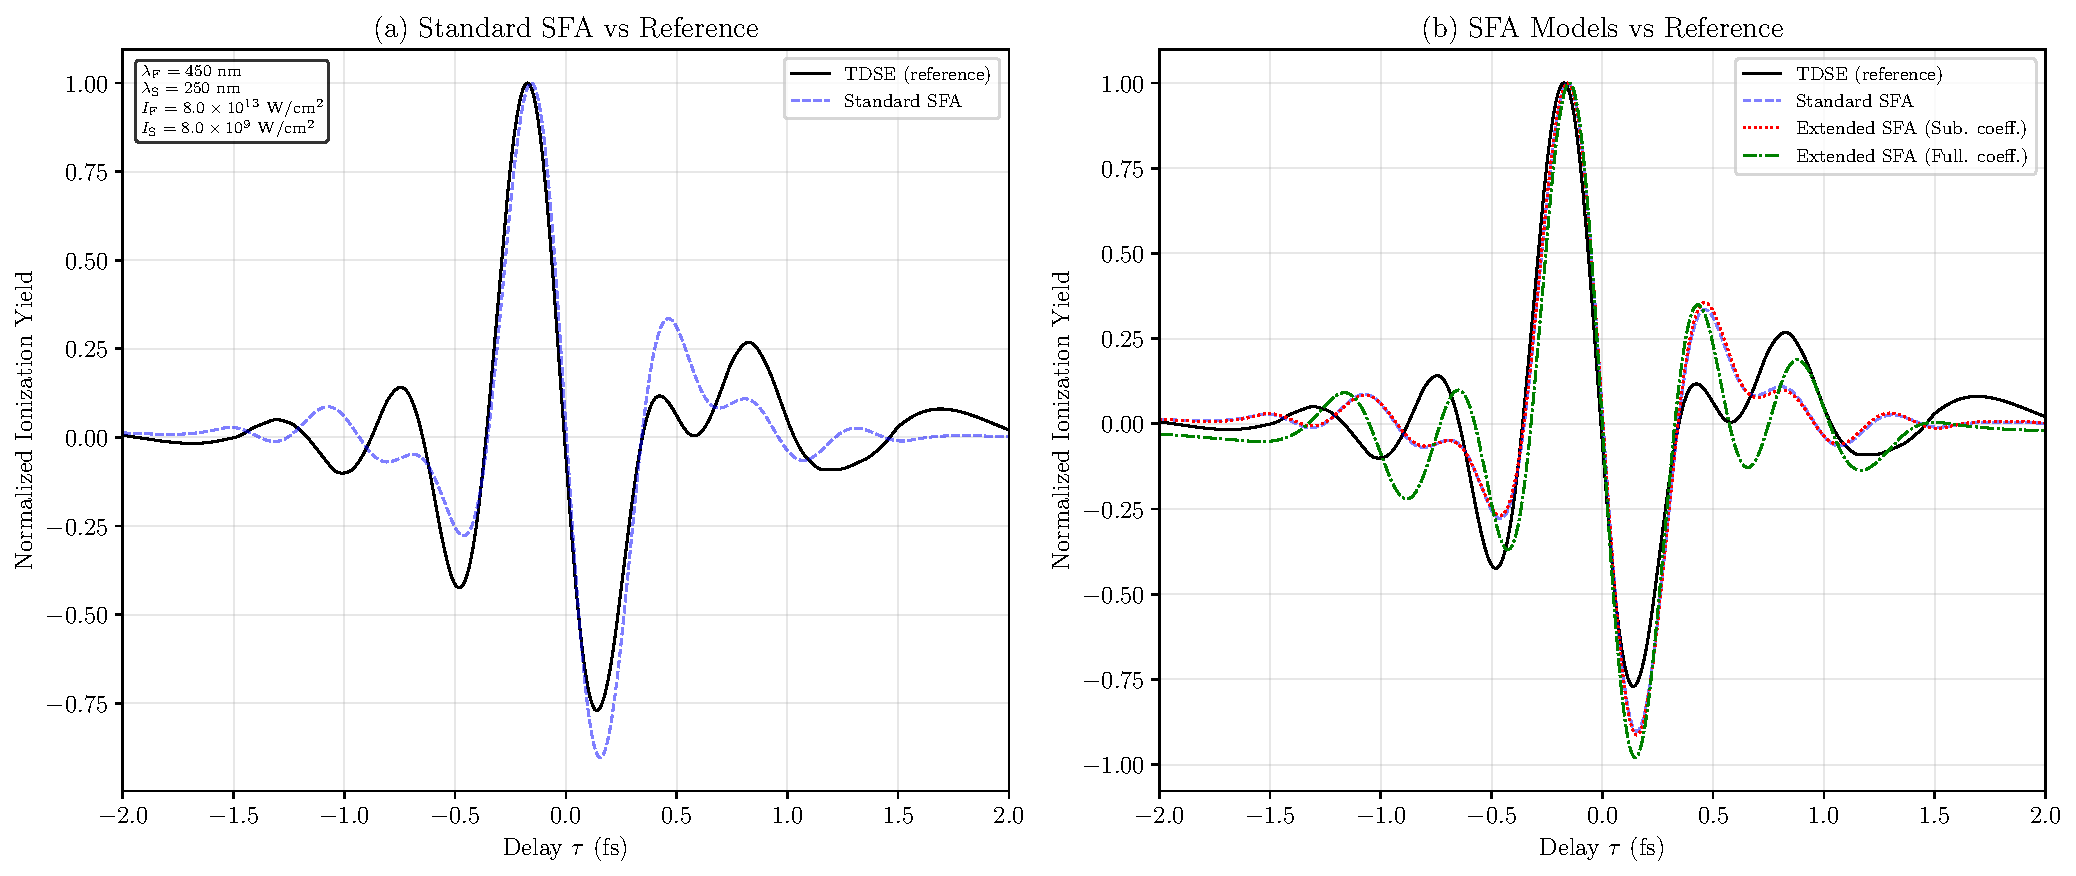
\includegraphics[width=1\textwidth]{figures/2plot_SFA-comparison_1_BA.pdf}
    \caption[Comparison of ionization dynamics predicted by SFA models and TDSE]{Comparison of ionization dynamics predicted between different SFA models and reference data from TDSE using TIPTOE simulations with transitions to excited states neglected.  
            (a) The standard SFA generally provides a reasonable reconstruction of the ionization dynamics, though certain features remain uncaptured.  
            (b) The extended model, with coefficients determined from solving the TDSE in the subspace, exhibits slight improvement. However, when coefficients from the wavefunction restricted to the subspace are used, no significant change or improvement in the dynamics is observed compared to the standard SFA.}  
    \label{fig:tiptoe_sfa_comparison}
\end{figure}

\paragraph{Stark shift or distortion of ground state}
As mentioned in Chapter 2, when ionization is `turned off' so the wavefunction remains within the subspace of bound states, two major physical effects are carried by the coefficient $c_0(t)$: the Stark shift and the distortion of the ground-state probability amplitude. By using only the phase of $c_0(t)$, the influence of the Stark shift can be isolated: \begin{equation} c_n(t) = |c_n(t)|e^{i \phi_n(t)} \rightarrow c_n(t) = e^{i \phi_n(t)} \end{equation} However, this approach is valid only for coefficients obtained by solving the TDSE for the wavefunction restricted to bound states, not for the `Full' approach.

\medskip
The results using only the phase of the coefficients are shown in figure \ref{fig:tiptoe_rate_stark}(a).
Nearly all improvement in ionization dynamics observed with the full Hilbert space coefficients can be attributed to changes in the phase, corresponding to energy level variations over time, while the coefficient amplitudes play a negligible role.
As the extended SFA results with coefficients from the subspace showed no improvement, it remains unclear from this plot whether the phase or amplitude dominates.

\medskip
Initially, it might appear that the improvement in the full Hilbert space TIPTOE result originates from the Stark effect, as suggested by equation \eqref{eq:ac_stark_shift}.
However, since the Stark effect must be present in both the subspace and full Hilbert space approaches, this provides strong evidence that the Stark effect plays only a minor role in subcycle ionization dynamics.
It should be noted that equation \eqref{eq:ac_stark_shift} is valid only for a wavefunction restricted to bound states, which is not the case in the `Full' approach.

% \medskip
% Figure \ref{fig:tiptoe_rate_stark}(b) and \ref{fig:tiptoe_rate_stark}(c) supports this with further detail.
% \medskip
% Furthermore, the ionization yield of the extended SFA models in \ref{fig:tiptoe_rate_stark}(b) is slightely lower than predicted from plain SFA, which can be interpeted as stark shift and ground state distortion makes it `harder' or `less likely' for the electron to get ionized.
% Therefore, for the electron with the full hilbertspace coefficients it should be harder aas well when including stark shift.
% However, \ref{fig:tiptoe_rate_stark}(b) shows the exact opposite, indicating the the significant change in the rate is something different than stark shift.

\medskip
This observation is further supported by the details shown in Figure \ref{fig:tiptoe_rate_stark}(b) and \ref{fig:tiptoe_rate_stark}(c).
The phase of the `Sub' coefficients appears to have a slightly larger impact than their magnitude, though this does not result in any meaningful change in the ionization dynamics shown in \ref{fig:tiptoe_rate_stark}(a).
In contrast, the phase of the coefficients associated with the wavefunction in the full Hilbert space leads to a significant change in the ionization rate, while the distortion in the ground state plays a relatively minor role.
When only the magnitudes of the coefficients are compared, the rates are similar, which supports and validates previous arguments.

\medskip
Additionally, the ionization yield predicted by the extended SFA models in \ref{fig:tiptoe_rate_stark}(b) is slightly lower than that of standard SFA, suggesting that the Stark shift and ground state distortion make ionization ‘harder’ and less probable for the electron.
If this interpretation holds, the electron with the full Hilbert space coefficients should also exhibit reduced ionization when the Stark shift is included.
However, \ref{fig:tiptoe_rate_stark}(b) shows the opposite behavior, indicating that the significant change in the rate is attributable to factors other than the Stark shift.

% \medskip
% In summary:
% \textcolor{red}{When only the Stark effect of the ground state is considered within the strong-field approximation, while determining the coefficients by solving the TDSE in the full Hilbert space, the phase of the ionization dynamics in the off-cycle region of the laser pulse is reconstructed more accurately than when only the distortion of the ground state is taken into account.}

\begin{figure}[htbp]
    \centering
    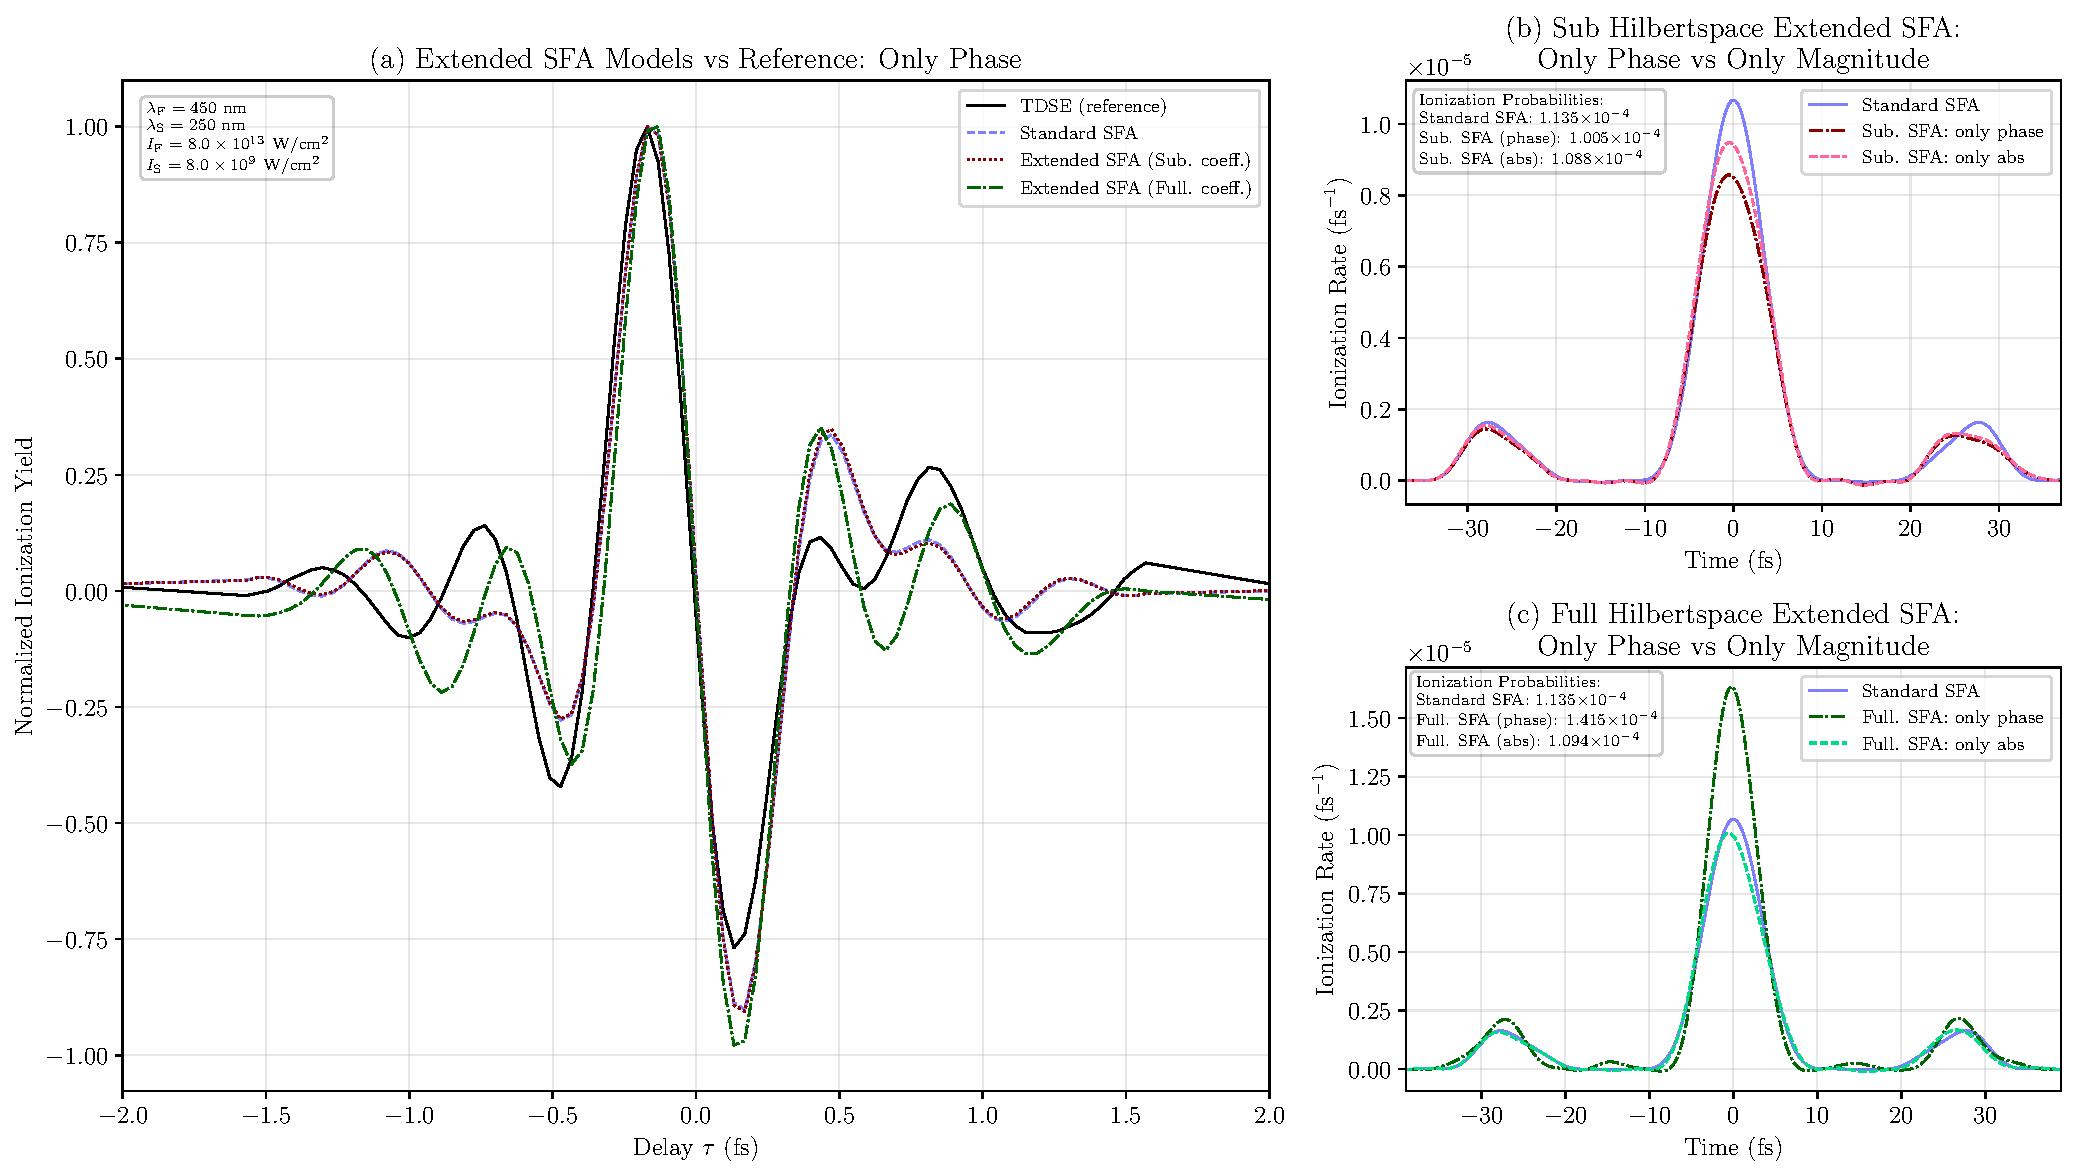
\includegraphics[width=0.99\textwidth]{figures/3plot_stark-comparison_1_BA.pdf}
    \caption[Impact of phase and magnitude of the coefficients on TIPTOE simulations and ionization rates]{Impact of phase and magnitude of the coefficients on TIPTOE simulations and ionization rates for fundamental pulse with transitions to excited states neglected. (a) When only the phase from the coefficients obtained by solving the TDSE in the full Hilbert space is used, an improvement in reconstructing ionization dynamics is observed, while the magnitude of the coefficients appears to have minimal impact. (b) Both the phase and the magnitude of the coefficients are found to have little impact on the ionization rate, though the phase shows slightly more influence. The phase can be interpreted directly as the Stark shift, as suggested by equation \eqref{eq:ac_stark_shift}. (c) The magnitude is observed to have a similar influence on the ionization probability as the subspace approach. However, when only the phase of the coefficients from the full Hilbert space is used, a significant difference compared to (b) is observed. This indicates that the change in the ionization rates is not attributable to the Stark effect.}
    \label{fig:tiptoe_rate_stark}
\end{figure}

\paragraph{Where does the difference come from?}
The previous paragraph raises the question of where the improvement between standard SFA and extended SFA with full Hilbert space coefficients originates, if it is not due to the Stark shift or distortion of the ground-state probability amplitude.
It should be noted that this is not the focus of the thesis, and thus no definitive answer is provided.
However, the difference must arise from effects that manifest in the phase of the coefficients, i.e., in the change of the ground-state energy level over time. Furthermore, this difference is \emph{only} observable when the wavefunction is allowed to ionize, meaning the TDSE is solved in the full Hilbert space.
Possible explanations include the influence of the Coulomb potential on ionization dynamics or other effects that are captured by a numerical solver but not by a simple system of ODE's.

\section{Difference in Ionization Yield between SFA and TDSE}
As mentioned in Chapter 3, the ionization yield of the TIPTOE simulations in figures \ref{fig:tiptoe_sfa_comparison} and \ref{fig:tiptoe_rate_stark}(a) is normalized to better visualize the actual differences.
Further, since the primary focus lies on the dynamics rather than the absolute ionization yield, the normalization is performed according to \eqref{eq:tiptoeprop_normalized}.
However, in the non-normalized plot, it can be observed that the numerical solution of the TDSE predicts an ionization probability orders of magnitude higher than that of the SFA model.
Additionally, small changes in the delay of the signal pulse lead to larger variations in the TDSE results compared to the SFA results, indicating that the `reference' TIPTOE result is more sensitive to changes in the laser field.

The first observation can be attributed to the fact that in the SFA model, it is assumed that the electron occupies a continuum state after ionization, meaning it no longer experiences the Coulomb potential.
This is, of course, a strong assumption and significantly more `difficult' for the electron to achieve.
For this approximation to hold, the laser must effectively `catapult' the electron out of the atom.
Consequently, the overall ionization yield predicted by the SFA model is much lower than that of the TDSE.
Second, the numerical solution of the TDSE captures a broader range of dynamics and physical effects during the ionization process.
Various processes can occur during this time, which may explain why the ionization yield in the TDSE is more sensitive to changes in the electric field.

While these observations are interesting, they align with the theoretical foundations of the SFA model.
To confirm that the discrepancies arise solely from the core assumptions of the SFA model (i.e., the treatment of the final state as a continuum state), other possible explanations must be ruled out.
The extended SFA model proposed in this thesis may provide insights into this question.
During this research, significant effort has been dedicated to implementing the extended SFA model, particularly to incorporate excited states.
However, due to time constraints, conclusive results on this matter could not be obtained.

Preliminary TIPTOE results suggest that including excited states in the SFA rate partially reduces the order-of-magnitude discrepancy between the SFA and TDSE predictions.
Additionally, the cross-coupling terms in \eqref{eq:sfa_rate_improved} (i.e., $n_1 \neq n_2$) appear to contribute significantly to the ionization rate.
Furthermore, the previously discussed importance of the energy shift in the phase also applies to excited states.
The energy level shifts of excited states have a more pronounced effect on the ionization rate than changes in the probability amplitudes of the coefficients.
The observed changes in the ionization yield magnitude, potentially arising from the inclusion of excited states in the extended SFA model, may primarily stem from the dipole transition matrix elements.
For instance, this could be explained by the laser pulse first exciting the electron to, say, the $3p$ state before ionizing it, leading to a higher overall ionization probability due to additional pathways.
However, this hypothesis could not be fully verified here.
These indications remain speculative and should not yet be considered definitive results.





% As mentioned in Chapter 3, the Ionization yield in \ref{fig:tiptoe_sfa_comparison} is normalized, to see the actual difference better.
% Further, because we are mostly interested in the dynamics and not the plain ionization yield, its normalized according to \eqref{eq:tiptoeprop_normalized}.
% However, in the not normalized plot, one could see that the numerical solution of the TDSE is predicting a ionization probability orders of magnitude higher than the SFA model.
% In addition to that, small changes in the in the delay of the signal pulse leads to bigger changes in the TDSE results than the SFA results, so the `reference' TIPTOE result is much more sensitive to changes in the laser field.
% First observation can be interpreted by the fact that in SFA we are assuming, the electron sits in a continuum state after ionization so the elecotrn does not `feel' the coulomb potential anymore.
% This is of course a very strong assumption, any much `harder' to achcieve for the electron. 
% Imagine the laser has to really catapult the electron out of the atom to make this assumption approximately valid.
% Therefore the overall ionization yield from the SFA model is much lower than the one from the TDSE.
% Second, the numerical solution of the TDSE captures much more dynamics and physical effects of the ionization process.
% Many different processes can happen during that time, and that could justify why the ionization yield of the TDSE is much more sensitive to changes in the elcetric field.

% Both these observations are interesting, but can be expected from how the SFA model is constructed.
% To make shure that the differences really do come from the `fundamentals' of the SFA model (i.e. the assumption that the final state is a continuum state), one has to make shure that is the only possible option for the differences.
% The extended SFA model described in this thesis may give promising insights into this question.
% During the research for this thesis, much work has gotten into the implementation of the extended SFA model, such that it incorparates also excited states .
% Unfortunately, due to the limited time frame, I can not present certain results for this question. 
% Latest TIPTOE results indicate that including excited states in the SFA rate help to a certain extend the difference in the order of magnitude between SFA and TDSE.
% Also the cross-coupling terms in \eqref{eq:sfa_rate_improved} (i.e. $n_1 \neq n_2$) seems to have a significant contribution to the ionizatiion rate.
% Furthermore, previous discussed results about the importance of the stark shift applies to excited states as well.
% The shift in the energy level of the excited states playes a more significant role for the ionization rate than changes in the probability ampltidue of the coefficients.
% The indicated changes in the order of magnitude of the ionization yield that could come from including excited states in the extended SFA model is could primarily coming from the dipole transition matrix elements.
% For example this could be explained by the lase rpulse exciting the elctron to for isnatnce the 3p state and later ionizing it.
% This will result in a much hgiher ionization probability overoll since more is possible.
% However, this could not be shown here.
% But these are not really results, only some hints.















% On the left plot we see that tRecX is still orders of magnitude larger than the SFA results. 
% However, with excited states it goes in the right direction as can be seen on the right plot. 
% For three excited sates there is not much imporvement visible.
% Unfortunately, the results are no where close to the tRecX measurements. That indicates that there is some physics missing in the SFA model.
% If its not the excited states, the it must be something else.
% And because the change is so big it has to be something more fundamental.
% The first idea is that the interaction with the coulomb potential after ionization cannot be completely neglected, as it is done in the SFA model.
% Even though it is counterintuitive, becasue if the coulomb potential is still noticable for the electron after ionization, why would it increase the results we are seeing??????
% But this is in principle what our simulations are telling us. We can argue that we have two different ways of calculating the coefficients (ODE and tRecX) and the reproduce the same result.

% However it indicates that real ionization propabilities do have some characterisitcs that the improved SFA model does not capture.

% One also should make clear what the ODE coefficients do not capture. First, I implemented the code such that it ignores transitions not allowed by the dipole selection rules.

% So in principle, assuming my SFA modification was correct the TIPTOE results tell us that the coulomb potential is not negligible after all. 
% Maybe because the laser is not that intense (multiphoton ionization).
% But its difficult to test that because if I increase the laser intensity, the approximations I made with the coefficients is not valid anymore.

% Looking at not normalized results, tRecX is much more sensitive to the shift of probe and pump pulse, while excited SFA coefficients are not
% Maybe because tRecX takes into account all the dynamics and effects inside an atom, while excited SFA coefficients does not care that much.
% I would expect with tRecX coefficients more sensitive than with ODE coefficients???

% \section{Influence of Stark Shift and Polarisation}
% The Stark effect is the shift of the energy levels of an atom or molecule due to the presence of an external electric field.

% \begin{figure}[H]
%     \centering
%     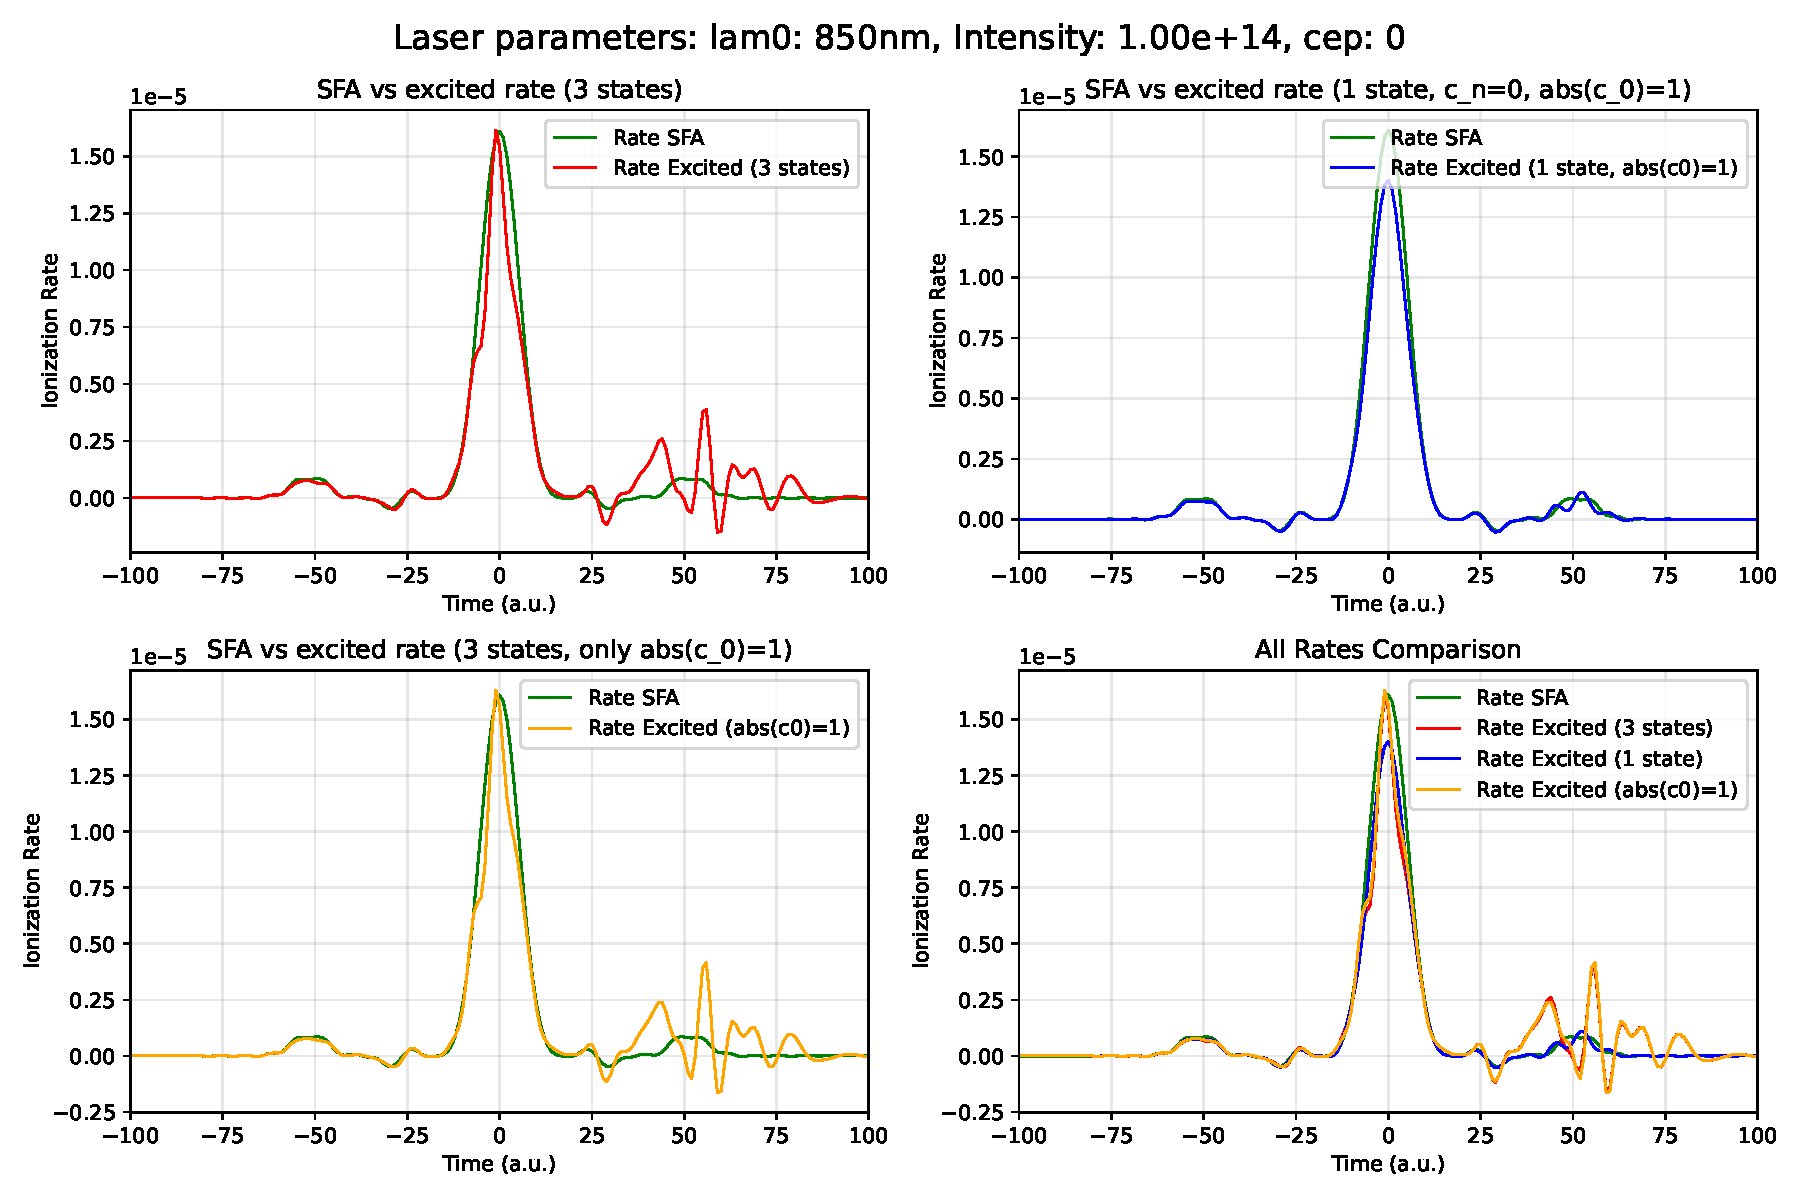
\includegraphics[width=0.9\textwidth]{figures/rate4_850_1.00e+14_onlystark.pdf}
%     \caption{stark effect}
%     \label{fig:starkeffect}
% \end{figure}

% Naiv: Stark effect changes energy in electron so its "harder" to ionise, thats why blue curve goes down (when excitedStates=1). 
% But thats not certainly the case because of stark effect, thats why only set absc0 to 1 and phase remains. 
% Example with oszillations with time dependent resonance frequency, and external force not at resonance but coincidence with oszillator resonance frequency so this may cause it.

% \bigskip
% Stark shift doesnt seem to have much contribution (sadly) but at least more than the polarisation of the ground state.

% Lets investigate the influence of first coefficient, nothing more. Only the phase has a contribution, the amplitude is not important.
% Thats because the amplitude determines something occupation propabilitiy, but the phase is $e^{-iEt}$ and if $E$ is shifted by a bit you can isolate it by just using purely the phase.\\
% Top right is the isolated stark effect








% \section{Laser Fields}
% Lorem ipsum dolor sit amet, consetetur sadipscing elitr, sed diam nonumy eirmod tempor invidunt ut labore et dolore magna aliquyam erat, sed diam voluptua. At vero eos et accusam et justo duo dolores et ea rebum. Stet clita kasd gubergren, no sea takimata sanctus est Lorem ipsum dolor sit amet. Lorem ipsum dolor sit amet, consetetur sadipscing elitr, sed diam nonumy eirmod tempor invidunt ut labore et dolore magna aliquyam erat, sed diam voluptua. At vero eos et accusam et justo duo dolores et ea rebum. Stet clita kasd gubergren, no sea takimata sanctus est Lorem ipsum dolor sit amet.


% \begin{equation}
%     \partial_t u = \mathcal{H}(t)  \lambda 
% \end{equation}

% \begin{figure}[H]
%     \centering
%     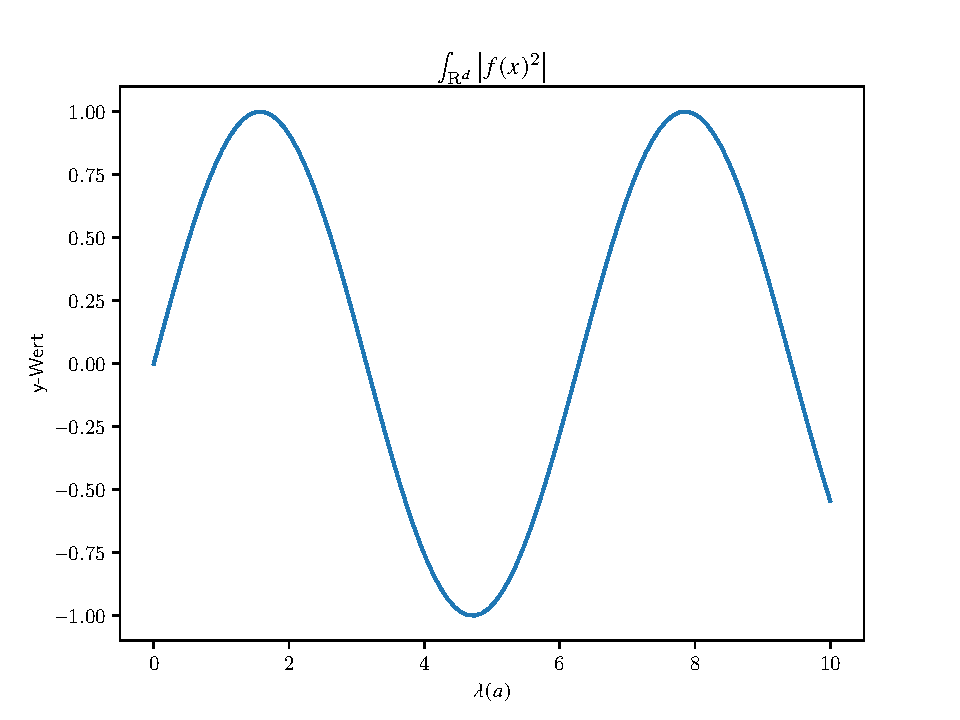
\includegraphics[width=0.5\textwidth]{figures/plot.pdf}
%     \caption{Sine function}
%     \label{fig:sinus}
% \end{figure}



% \begin{equation*}
%     \partial \A = \B
% \end{equation*}

% \medskip

% \begin{equation}
%     \int_{\R^d} \abs{f(x)}^2 \dd x = \int_{\R^d} \abs{\F f(\xi)}^2 \dd \xi
% \end{equation}

% \medskip

% \begin{equation}
%     %schrödinger equation
%     \ii \partial_t u = \mathcal{H}(t) \Ket{a} \lambda 
% \end{equation}

% \begin{equation}
%     \gimel \overrightarrow{a} \cos \mathrm{cos} \Rightarrow \Longrightarrow \nearrow 
% \end{equation}